\section{Development Toolchains}
PopcornSAR is a specialized Software-Defined Vehicle (SDV) tool and platform vendor focusing on the AUTOSAR Adaptive Platform to support automotive projects through advanced tools and engineering services. Their core design tool, {AutoSAR.io}, serves as a comprehensive authoring environment for modeling and configuring both Adaptive and Classic AUTOSAR platforms, offering features like graphical modeling, code generation, and interoperability with formats such as CAN DBC and COVESA VSS. This is complemented by {PARA}, an independently developed software framework designed for High-Performance Computing (HPC) that provides essential Adaptive AUTOSAR Functional Clusters---including communication (\texttt{ara::com}), execution management (\texttt{ara::exec}), and functional safety (\texttt{ara::phm})---to enable flexible and secure vehicle system development.

\begin{figure}[h]
    \centering
    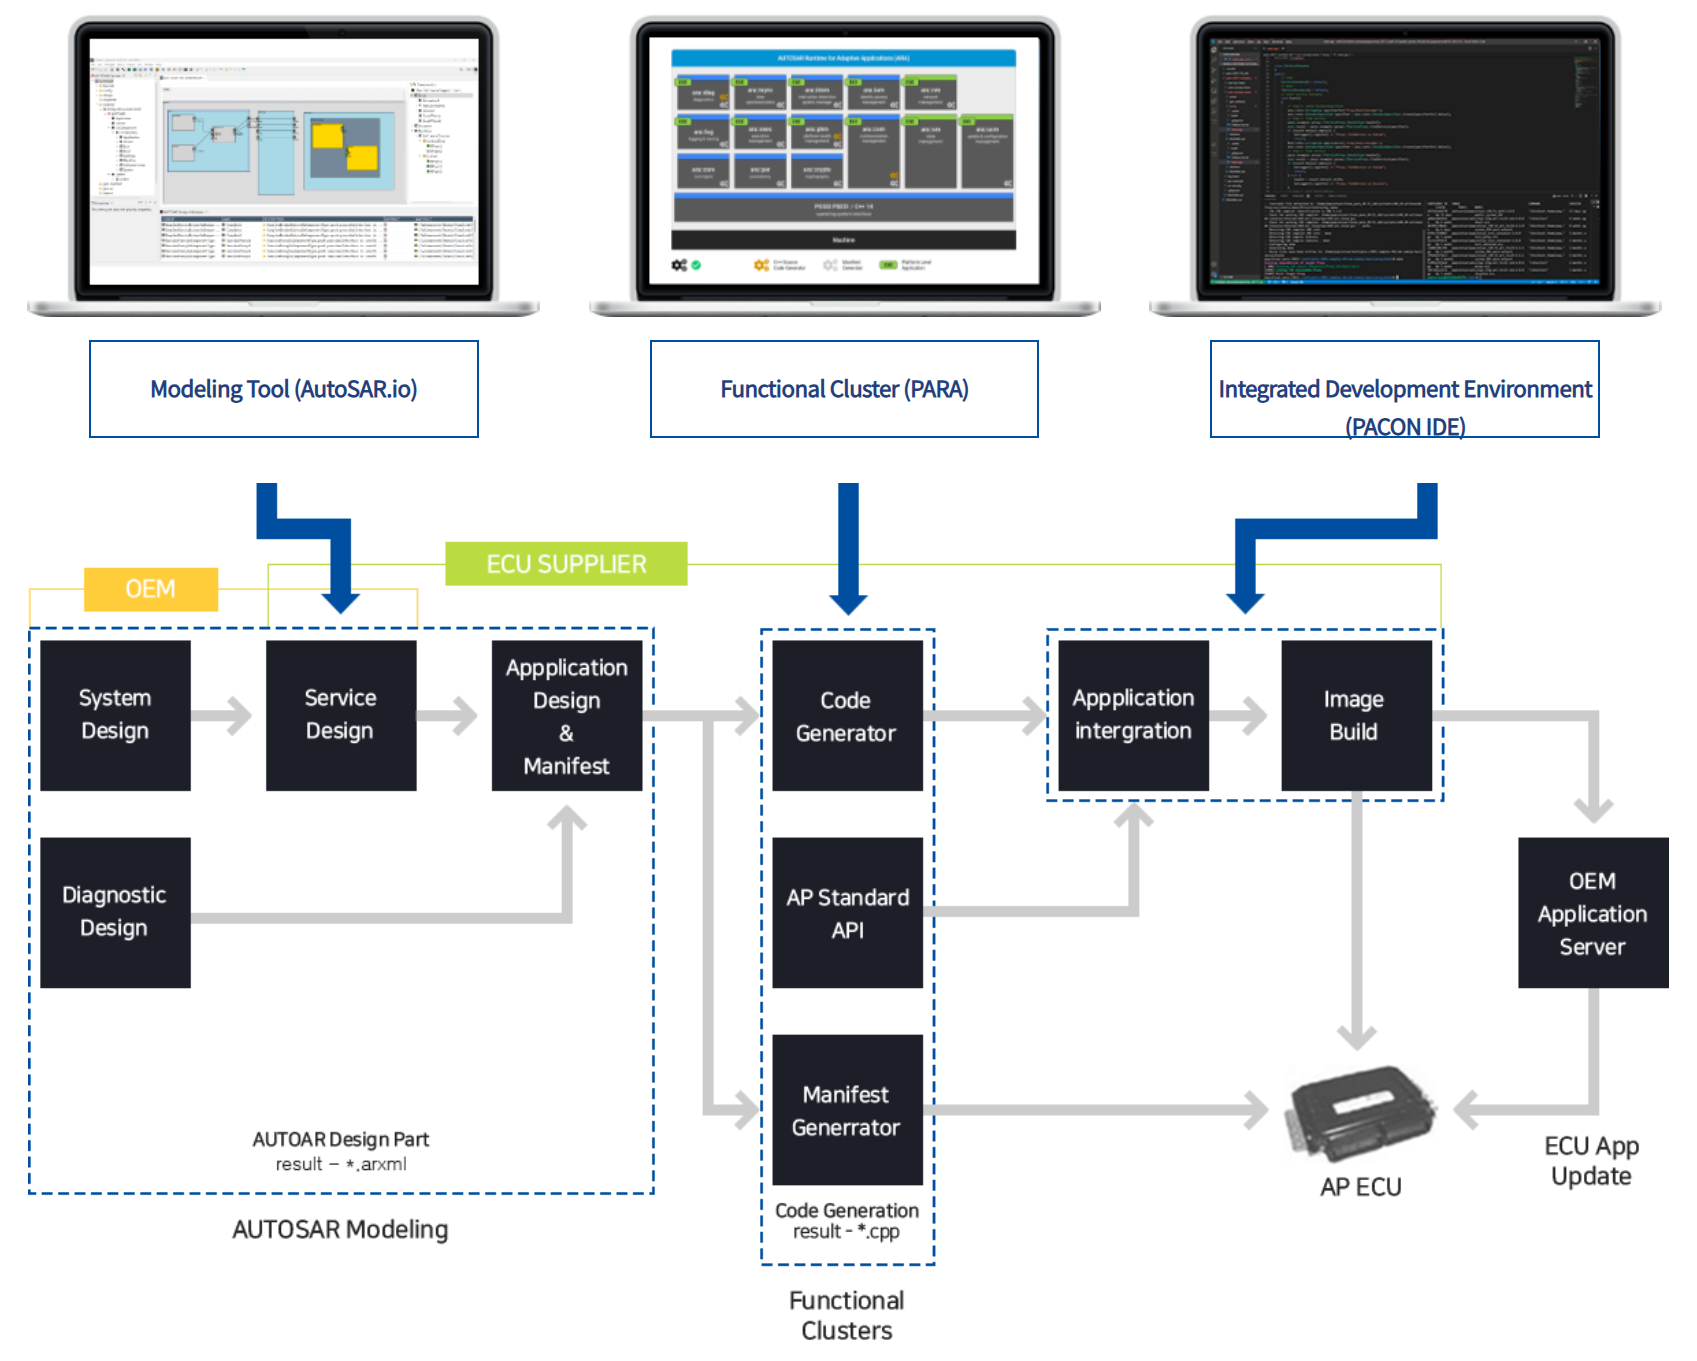
\includegraphics[width=1\textwidth]{Images/chapter2/tool_breakdowntool.png}
    \vspace{0.5cm}
    \caption{PopcornSAR Toolchain Breakdown \cite{popcornsar_intro}}
    \label{fig:popcornsar_toolchain}
\end{figure}

\subsection{AutoSAR.io}

AutoSAR.io is a powerful authoring tool developed by PopcornSAR, designed for the modeling and configuration of AUTOSAR projects within automotive systems. It serves as a comprehensive, future-proof development environment that supports the entire engineering spectrum, including System Architecture as well as both the Adaptive and Classic AUTOSAR Platforms. The tool is specifically built to empower customers in the efficient development of Software-Defined Vehicles (SDV), enabling them to significantly reduce complexity and accelerate the advancement of future automotive architectures.

Key features of AutoSAR.io include the capability to handle AUTOSAR System Design and the implementation of both Adaptive and Classic Platforms within a single tool. It streamlines the engineering process through graphical modeling for software components, internal behavior, and in-vehicle networks, complemented by a spreadsheet-style configurator and full support for the AUTOSAR methodology. The platform includes specialized designers for elements such as Adaptive Applications, Machines, Data Types, and Interfaces, along with ECU configuration for realtime environment (RTE), OS, and basic software (BSW). Additionally, AutoSAR.io functions as a robust code generator for AUTOSAR-compliant code and manifest files, and it offers seamless format conversion to integrate data models like CAN DBC, COVESA VSS, and existing ARXML into the AUTOSAR ecosystem.

\begin{figure}[h]
    \centering
    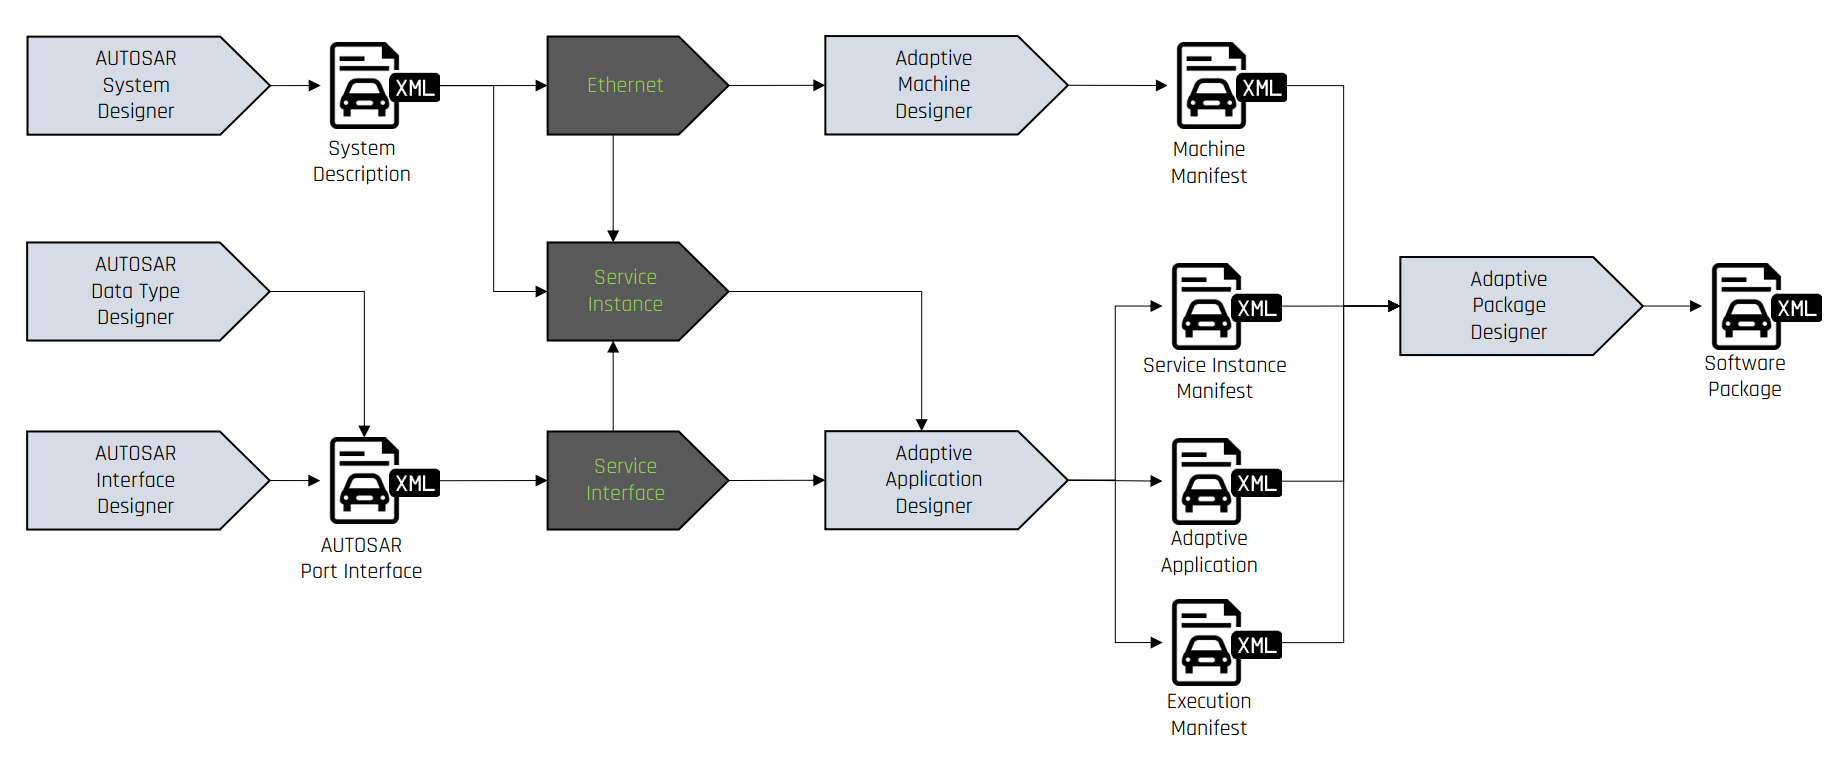
\includegraphics[width=1\textwidth]{Images/chapter2/aio_ap.png}
    \vspace{0.5cm}
    \caption{Adaptive Platform Workflow in AutoSAR.io \cite{popcornsar_intro}}
    \label{fig:autosar_io_ap}
\end{figure}


\begin{figure}[h]
    \centering
    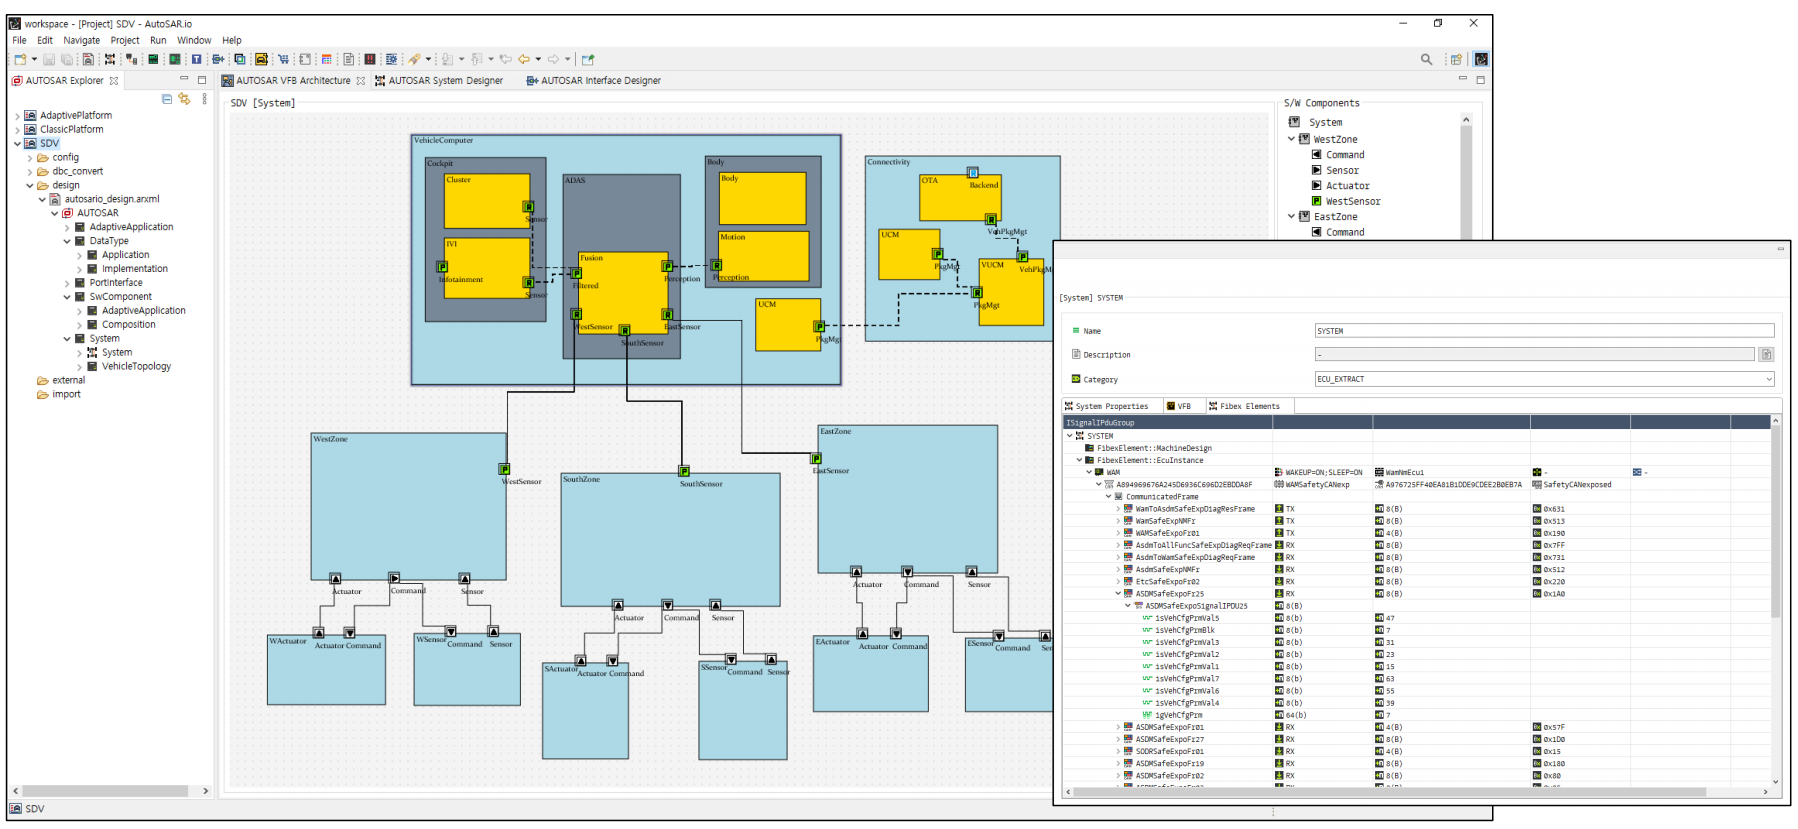
\includegraphics[width=1\textwidth]{Images/chapter2/aio_systemdesign.png}
    \vspace{0.5cm}
    \caption{AUTOSAR System Design in AutoSAR.io \cite{popcornsar_intro}}
    \label{fig:autosar_io_systemdesign}
\end{figure}

\begin{figure}[h]
    \centering
    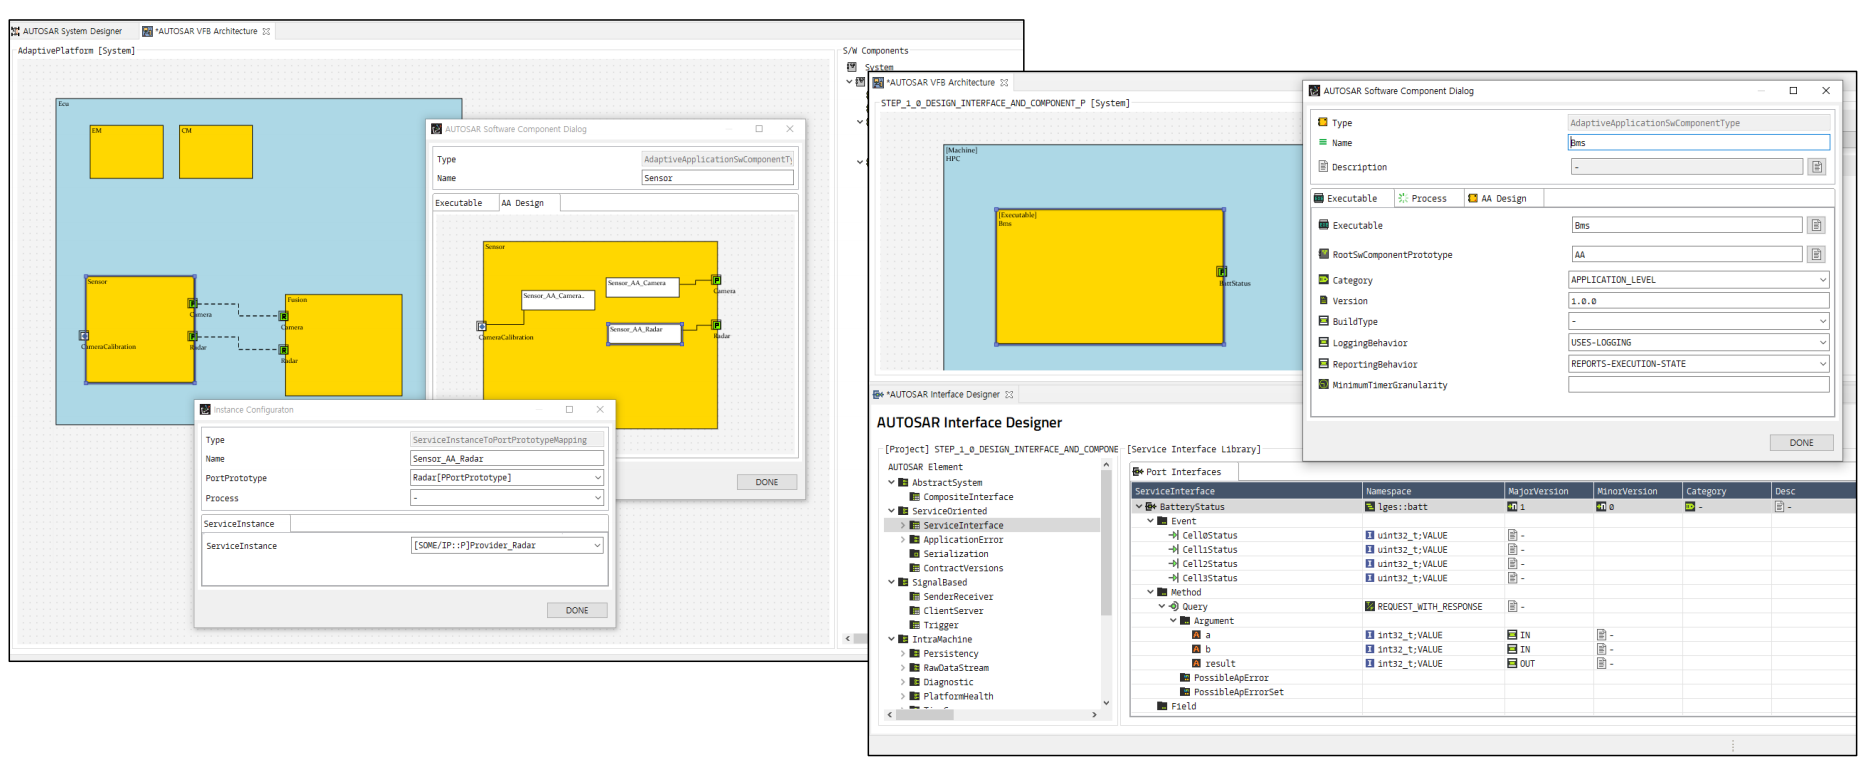
\includegraphics[width=1\textwidth]{Images/chapter2/aio_appldesign.png}
    \vspace{0.5cm}
    \caption{Application Design in AutoSAR.io \cite{popcornsar_intro}}
    \label{fig:autosar_io_appldesign}
\end{figure}


% \begin{figure}[h]
%     \centering
%     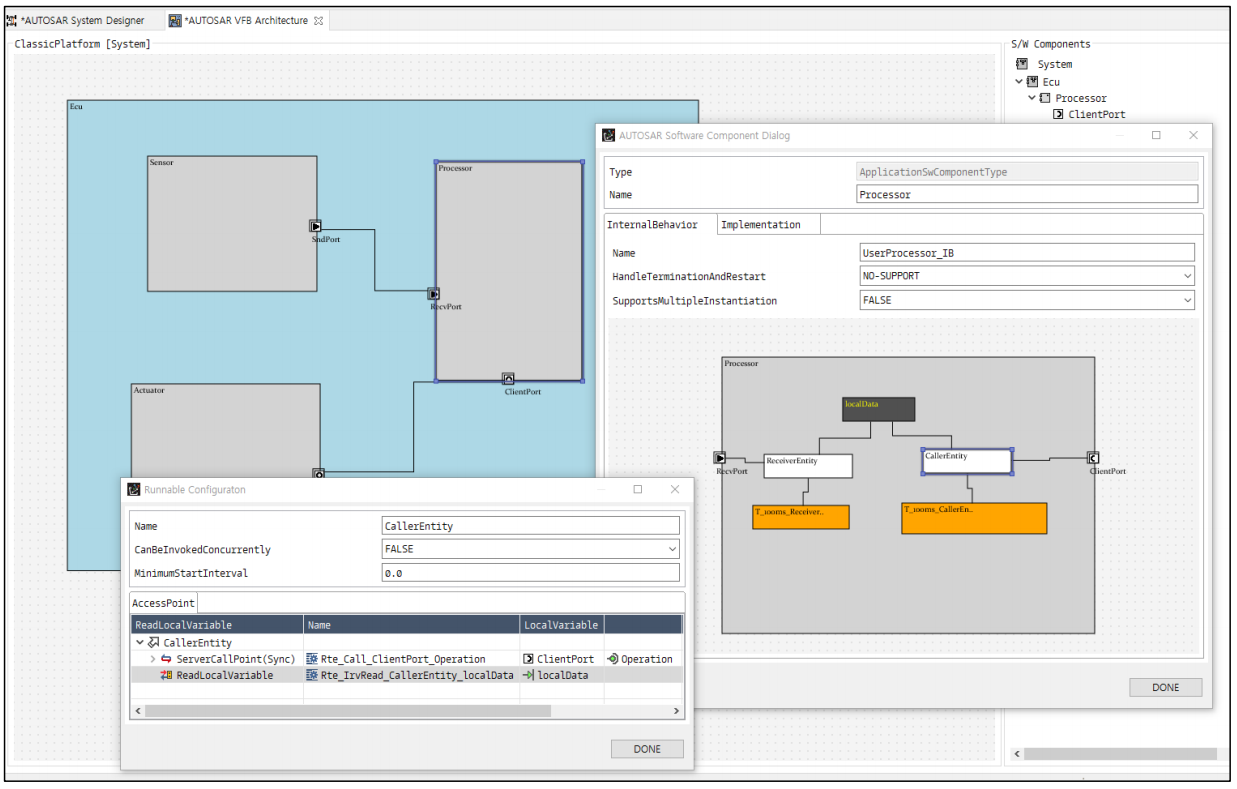
\includegraphics[width=1\textwidth]{Images/chapter2/aio_swdesign.png}
%     \vspace{0.5cm}
%     \caption{Software Component Design in AutoSAR.io \cite{popcornsar_intro}}
%     \label{fig:autosar_io_swdesign}
% \end{figure}

% \begin{figure}[h]
%     \centering
%     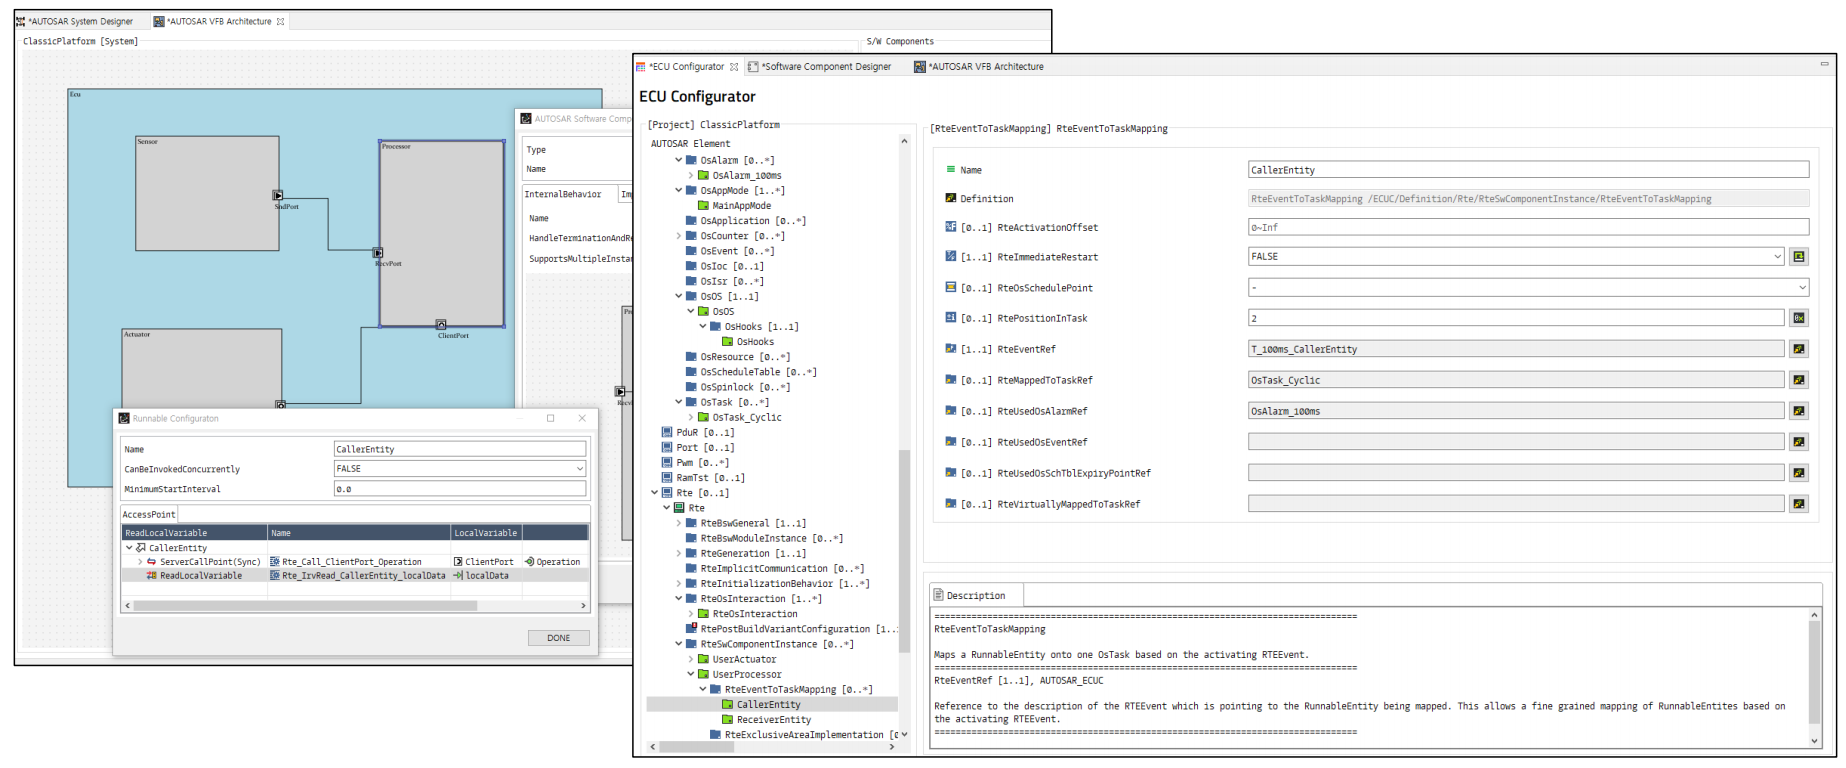
\includegraphics[width=1\textwidth]{Images/chapter2/aio_ecucfg.png}
%     \vspace{0.5cm}
%     \caption{ECU Configuration in AutoSAR.io \cite{popcornsar_intro}}
%     \label{fig:autosar_io_ecucfg}
% \end{figure}

AutoSAR.io is a powerful modeling tool that supports Code Generator of AUTOSAR-compliant code and manifest files. It streamlines development workflows while enabling full customization based on customer-specific requirements.

\begin{figure}[h]
    \centering
    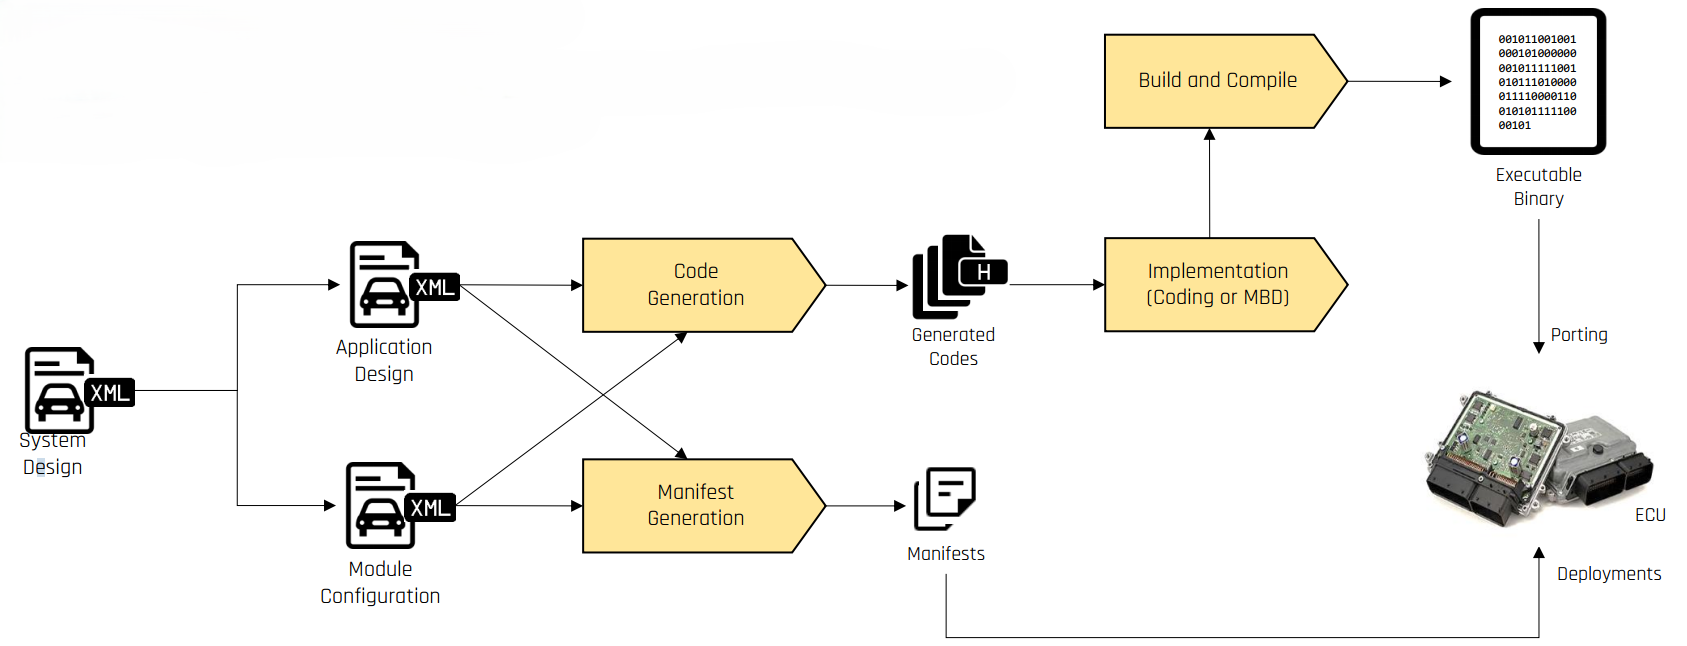
\includegraphics[width=1\textwidth]{Images/chapter2/aio_gen.png}
    \vspace{0.5cm}
    \caption{Code Generator Workflow in AutoSAR.io \cite{popcornsar_intro}}
    \label{fig:autosar_io_codegen}
\end{figure}

% AutoSAR.io supports seamless conversion of various data model formats such as CAN DBC, COVESA VSS, and AUTOSAR ARXML into AUTOSAR-compliant models. This allows smooth integration of existing vehicle data assets into the AUTOSAR eco-system.

% \begin{figure}[h]
%     \centering
%     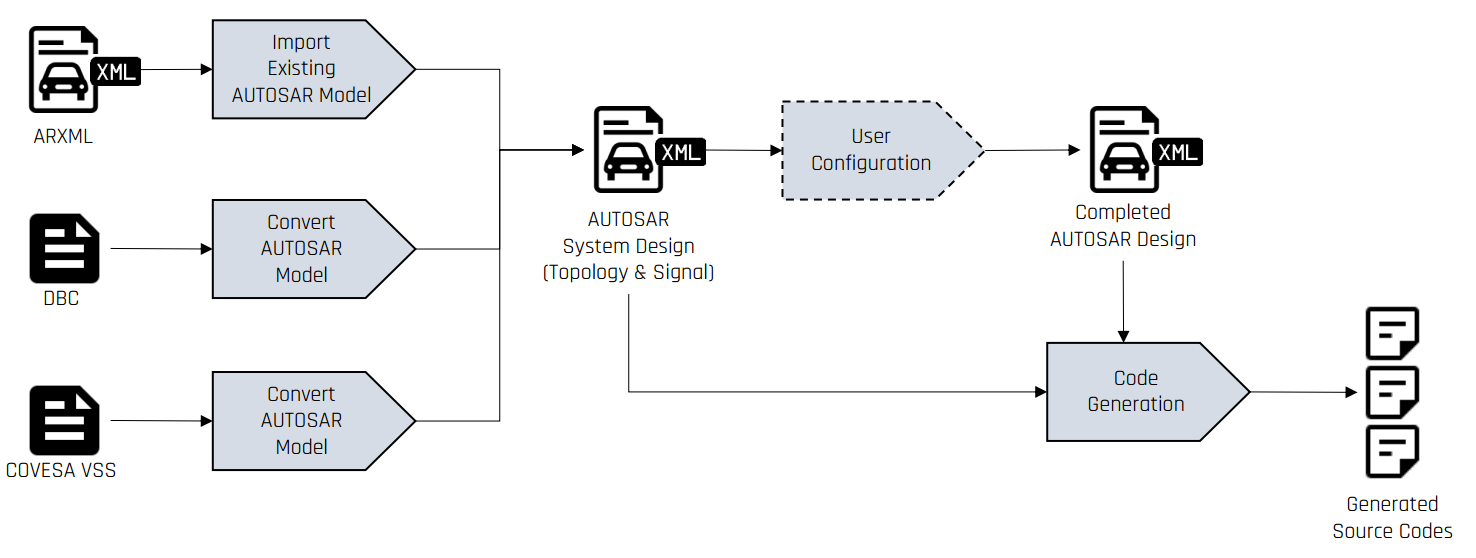
\includegraphics[width=1\textwidth]{Images/chapter2/aio_othergen.png}
%     \vspace{0.5cm}
%     \caption{Other Data Format Conversion Workflow in AutoSAR.io \cite{popcornsar_intro}}
%     \label{fig:autosar_io_othergen}
% \end{figure}
\newpage
\subsection{PARA}

PARA is PopcornSAR's ASIL-B certified AUTOSAR Adaptive Platform software framework, explicitly engineered for automotive HPC to accelerate the development of SDV. It delivers a comprehensive SOA that seamlessly integrates traditional automotive functions with modern IT frameworks like ROS2 and AI. To ensure robust operation across critical ADAS and VCU applications, PARA provides a suite of specialized functional clusters: \texttt{ara::com} manages diverse communication protocols (SOME/IP, DDS, zero-copy IPC, and Signal-To-Service), \texttt{ara::exec} orchestrates safe application lifecycles, and \texttt{ara::phm} enforces ISO 26262-compliant health monitoring. Furthermore, the SDK incorporates rigorous security mechanisms (\texttt{ara::idsm}, \texttt{ara::crypto}), diagnostic capabilities (\texttt{ara::diag}), secure Over-The-Air updates (\texttt{ara::ucm}), and legacy signal-based bridging (\texttt{para::sigcom}, \texttt{ara::aag}) to form a highly scalable, secure, and future-proof automotive development ecosystem.


\begin{figure}[h]
    \centering
    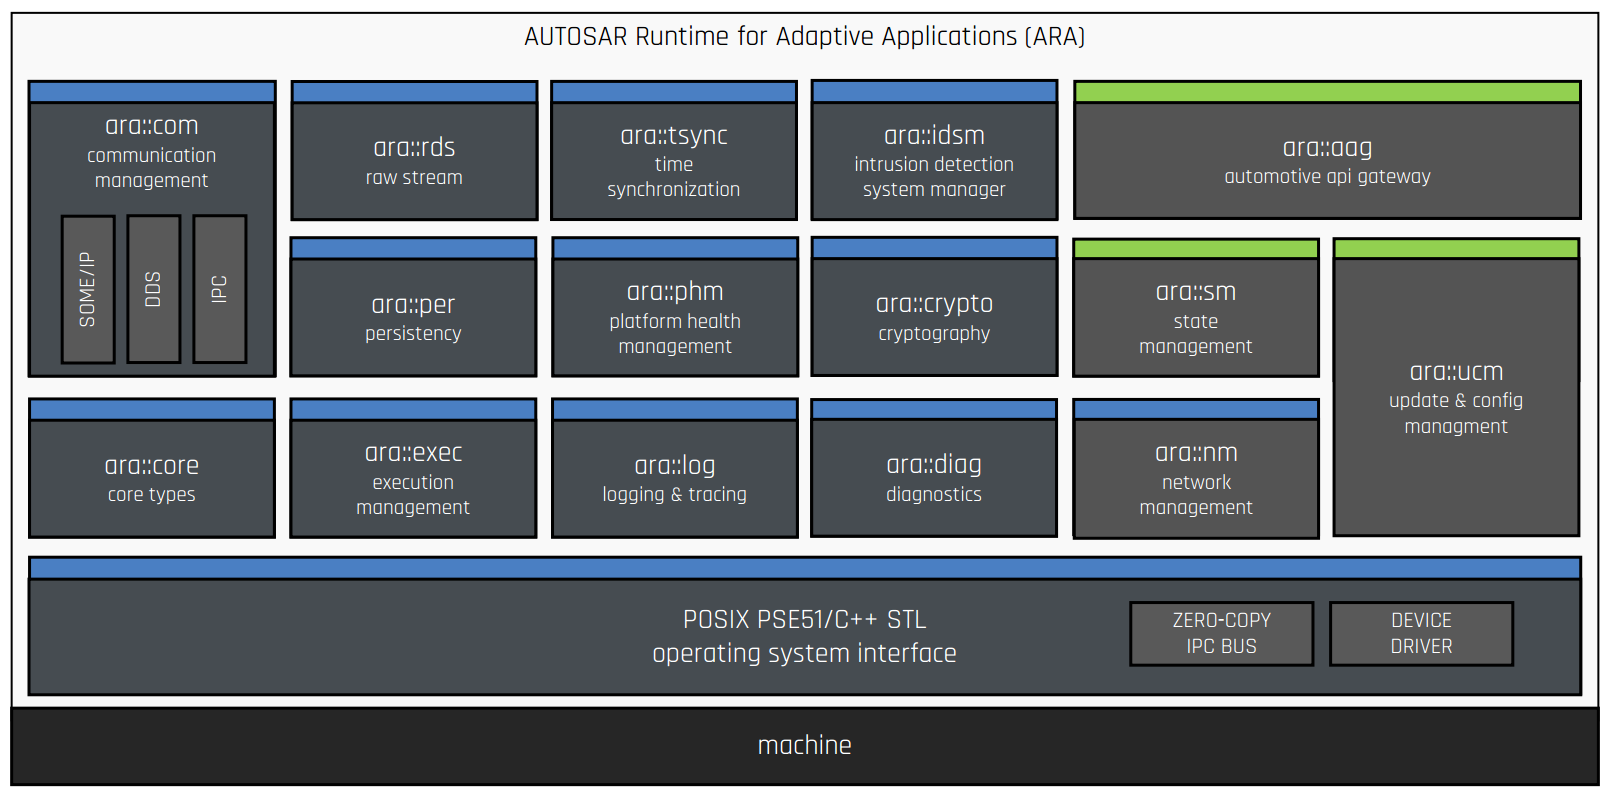
\includegraphics[width=1\textwidth]{Images/chapter2/para_basemodule.png}
    \vspace{0.5cm}
    \caption{Base Modules in PARA \cite{popcornsar_intro}}
    \label{fig:para_basemodule}
\end{figure}
\newpage
\paragraph*{Communication}(\texttt{ara::com})

\begin{figure}[h]
    \centering
    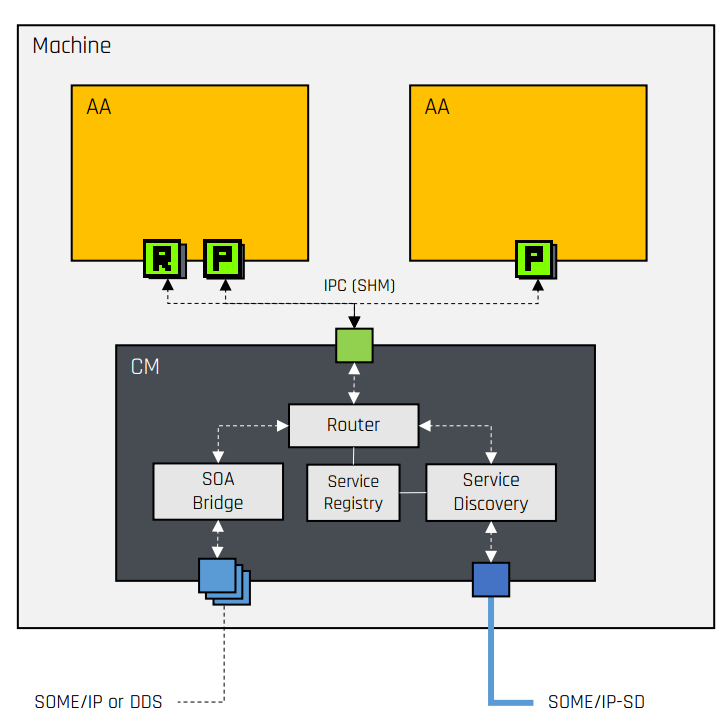
\includegraphics[width=0.5\textwidth]{Images/chapter2/para_com.png}
    \vspace{0.5cm}
    \caption{Communication in PARA \cite{popcornsar_intro}}
    \label{fig:para_com}
\end{figure}

PARA provides the complete product level for Service-Oriented Communication features. With PARA, \texttt{ara::com} provides full API and management for implementing service instances with application.

Some Protocols for SOA are supported in PARA like SOME/IP, DDS, and IPC (For Intra-machine).

PARA has base scheme for High-Performance IPC with zero-copy. 


\paragraph*{Execution Management}(\texttt{ara::exec})


\begin{figure}[h]
    \centering
    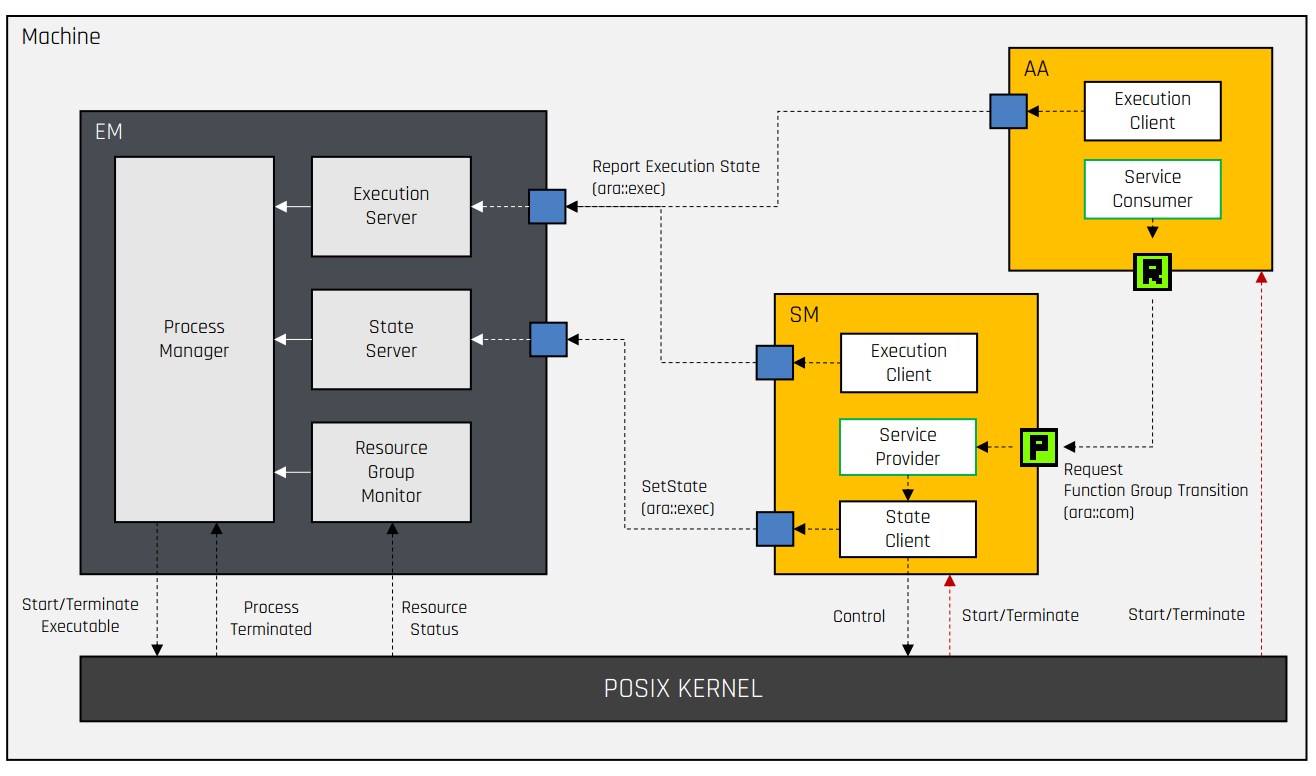
\includegraphics[width=0.8\textwidth]{Images/chapter2/para_exec.png}
    \vspace{0.5cm}
    \caption{Execution Management in PARA \cite{popcornsar_intro}}
    \label{fig:para_exec}
\end{figure}

With PARA, ara::exec provides management of applications with your configured scenario with state, execution dependency and resource statues. It also supports safe starting and termination of applications and machine.

After introducing the toolchain used to configure and generate Adaptive AUTOSAR applications, the following sections describe the AI models and inference runtime that provide the perception capability of the prototype.